\subsection{Montgomery Product}

Modular multiplications would involve trial division after the
multiplication step were it not for the algorithm know as Montgomery
product invented by Peter L. Montgomery \cite{Montgomery}.

The basic step and the property of the algorithm is computing the
residues modulo $N$.

\begin{defn}
  Define an radix $R$ such that $R R^{-1} - N N' = 1$. The residue
  $\overline{a}$ of $a$ is $\overline{a} = a R$
\end{defn}

\begin{thm}
  The algorithm for Montgomery reduction is
  \begin{algorithm}[hbt!]
    \caption{Montgomery reduction}
    \begin{algorithmic}
      \Function{Reduce}{$T$}
      \State $m \gets (T \bmod{R}) N' \bmod{R}$
      \State $t \gets (T + m N)/R$
      \If{$t \ge N$} \Return $t - N$
      \Else \, \Return $t$
      \EndIf
      \EndFunction
    \end{algorithmic}
  \end{algorithm}
\end{thm}
\begin{proof}
  Assume $T < R$, then
  \begin{align*}
      m & = T N' \\
    m N & = T N' N \\
        & = T R R^{-1} - T \\
        & = - T \bmod{R} \\
    t R & = T + m N \\
        & = T \bmod{N}
  \end{align*}
\end{proof}

To compute the Montgomery product, one can now apply the reduction to
the product of the reduced $\overline{a}$ and $\overline{b}$:
\begin{algorithmic}
  \Function{MontgomeryProduct}{$\overline{a}$, $\overline{b}$}
    \State $t \gets \overline{a} \cdot \overline{b}$
    \State \Return \Call{Reduce}{$t$}
  \EndFunction
\end{algorithmic}

Ko\c{c} goes a step further and inlines the reduction to see possible
optimizations when implementing the algorithm on multiple
architectures \cite{Koc}:

\begin{algorithm}[hbt!]
  \begin{algorithmic}
    \Function{MontgomeryProduct}{$\overline{a}$, $\overline{b}$}
      \State $m \gets (\overline{a} \cdot \overline{b} \bmod{R}) N' \bmod{R}$
      \State $t \gets (\overline{a} \cdot \overline{b} + m N)/R$
      \If{$t \ge N$} \Return $t - N$
      \Else \, \Return $t$
      \EndIf 
   \EndFunction
  \end{algorithmic}
\end{algorithm}

If such a primitive is provided on an architecture, the reduction then
becomes:

\begin{algorithm}
  \begin{algorithmic}
    \Function{MontgomeryReduce}{$T$}
      \State \Return \Call{MontgomeryProduct}{$T$, $R^2$}
    \EndFunction
  \end{algorithmic}
\end{algorithm}

Montgomery product eliminates the trial division. It does so at the
expense of computing the residues. However, these residues can be
precomputed in the beginning. Then, for a sufficient number of
Montgomery multiplications, the amortized cost is negligible. The
problem of computing the modular product is then given by:
\begin{enumerate}
\item Transform into the Montgomery domain
\item Compute the product in the Montgomery domain
\item Transform the result back into the integer domain
\end{enumerate}
This is also depicted in Figure \ref{fig:montpro_flow} where both paths
are shown when starting from the integer domain.

\begin{figure}[hbt!]
  \centering
  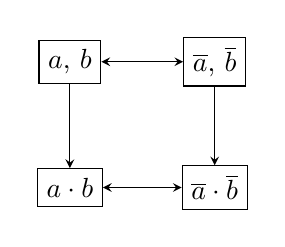
\begin{tikzpicture}[>=stealth]
    \tikzstyle{dom}=[rectangle,draw=black,thin,align=center]

    \node[matrix, column sep=1cm, row sep=1cm](matrix){
      \node[dom](intd){$a$, $b$}; & \node[dom](montd){$\overline{a}$, $\overline{b}$}; \\
      \node[dom](intpro){$a \cdot b$}; &\node[dom](montpro){$\overline{a} \cdot \overline{b}$}; \\
    };

    \draw[<->] (intd) -- (montd);
    \draw[->] (montd) -- (montpro);
    \draw[<->] (montpro) -- (intpro);
    \draw[->] (intd) -- (intpro);
  \end{tikzpicture}
  \caption{Montgomery product flow}
  \label{fig:montpro_flow}
\end{figure}

%%% Local Variables: 
%%% mode: latex
%%% TeX-master: "thesis"
%%% End: 
